\documentclass[11pt, letterpaper]{article}

% Fonts and Encoding
\usepackage[utf8]{inputenc}
\usepackage[T1]{fontenc}
\usepackage{lmodern} % High-quality Latin Modern vector font

% Math and Symbols
\usepackage{amsmath, amssymb, amsthm, amsfonts, mathrsfs, mathtools}

% Layout and Geometry
\usepackage{geometry}
\geometry{letterpaper, margin=1in}
\setlength{\parindent}{0pt}
\setlength{\parskip}{0.6em}

% Formatting and Graphics
\usepackage{graphicx, xcolor, enumitem, booktabs, array, tabularx}

% TikZ for Illustrations
\usepackage{tikz}
\usetikzlibrary{arrows.meta, positioning, shapes.geometric, calc, backgrounds, matrix}

% Clickable Links and TOC
\usepackage{hyperref}
\hypersetup{
    colorlinks=true,
    linkcolor=blue,
    filecolor=magenta,      
    urlcolor=cyan,
    pdftitle={Advanced Mathematics Topic},
}

% Theorem Environments
\newtheorem{theorem}{Theorem}[section]
\newtheorem{lemma}[theorem]{Lemma}
\newtheorem{proposition}[theorem]{Proposition}
\newtheorem{corollary}[theorem]{Corollary}
\theoremstyle{definition}
\newtheorem{definition}{Definition}[section]
\newtheorem{axiom}{Axiom}[section]
\newtheorem{example}{Example}[section]
\theoremstyle{remark}
\newtheorem{remark}{Remark}[section]

% Custom Commands (Enforced standard notation)
\newcommand{\R}{\mathbb{R}}
\newcommand{\N}{\mathbb{N}}
\newcommand{\Z}{\mathbb{Z}}
\newcommand{\Q}{\mathbb{Q}}
\newcommand{\E}{\mathbb{E}}
\newcommand{\Prob}{\mathbb{P}}
\newcommand{\F}{\mathcal{F}}

\title{\textbf{Mastering Orthogonal Sets and Projections}}
\author{Tashfeen Omran}
\date{\today}

\begin{document}

\maketitle
\tableofcontents
\newpage

\section{Comprehensive Introduction, Context, and Prerequisites}

\subsection{Core Concepts}
The study of \textbf{Orthogonality} in linear algebra generalizes the geometric concept of perpendicularity to $n$-dimensional vector spaces ($\R^n$). Two vectors $\mathbf{u}$ and $\mathbf{v}$ are orthogonal if their inner product (dot product) is zero: $\mathbf{u} \cdot \mathbf{v} = 0$. 

An \textbf{Orthogonal Set} is a collection of vectors where every distinct pair is orthogonal. If these vectors also have a unit length (norm of $1$), the set is called an \textbf{Orthonormal Set}. When such a set forms a basis for a subspace, it is called an orthogonal (or orthonormal) basis. These bases are incredibly powerful because they decouple linear systems, allowing us to compute coordinates (weights) independently without solving massive systems of equations.

\subsection{Intuition and Derivation}
The formula for the \textbf{Orthogonal Projection} of a vector $\mathbf{y}$ onto a vector $\mathbf{u}$ is derived directly from vector addition and the definition of orthogonality. We want to decompose $\mathbf{y}$ into two components:
\[ \mathbf{y} = \hat{\mathbf{y}} + \mathbf{z} \]
where $\hat{\mathbf{y}} = \alpha \mathbf{u}$ (a scalar multiple of $\mathbf{u}$) and $\mathbf{z}$ is orthogonal to $\mathbf{u}$. 
Since $\mathbf{z} \cdot \mathbf{u} = 0$, we substitute $\mathbf{z} = \mathbf{y} - \alpha \mathbf{u}$:
\[ (\mathbf{y} - \alpha \mathbf{u}) \cdot \mathbf{u} = 0 \implies \mathbf{y} \cdot \mathbf{u} - \alpha (\mathbf{u} \cdot \mathbf{u}) = 0 \implies \alpha = \frac{\mathbf{y} \cdot \mathbf{u}}{\mathbf{u} \cdot \mathbf{u}} \]
Thus, the projection is $\hat{\mathbf{y}} = \frac{\mathbf{y} \cdot \mathbf{u}}{\mathbf{u} \cdot \mathbf{u}} \mathbf{u}$.

\begin{center}
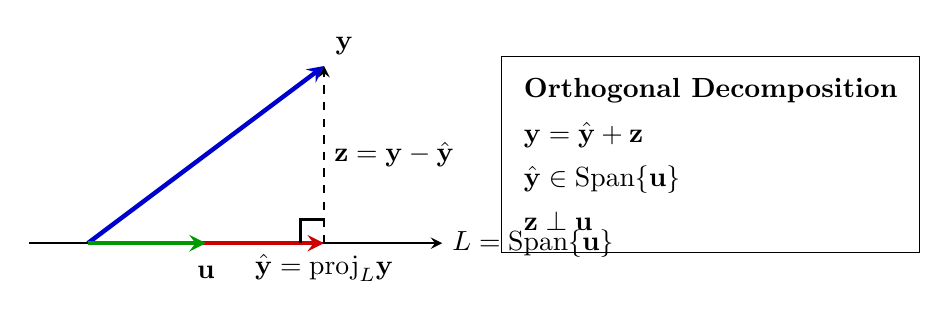
\begin{tikzpicture}[scale=1.5]
    % 1) Background (None needed here, but keeping protocol)
    % 2) Grid/Axes
    \draw[thick, ->, >=stealth] (-0.5, 0) -- (3, 0) node[right] {$L = \text{Span}\{\mathbf{u}\}$};
    % 3) Primary Plots
    \coordinate (O) at (0,0);
    \coordinate (Y) at (2, 1.5);
    \coordinate (Yhat) at (2, 0);
    \coordinate (U) at (1, 0);
    
    \draw[ultra thick, blue!80!black, ->, >=stealth] (O) -- (Y) node[above right, text=black] {$\mathbf{y}$};
    \draw[ultra thick, red!80!black, ->, >=stealth] (O) -- (Yhat) node[below, text=black] {$\hat{\mathbf{y}} = \text{proj}_L \mathbf{y}$};
    \draw[thick, dashed, ->, >=stealth] (Yhat) -- (Y) node[midway, right, text=black] {$\mathbf{z} = \mathbf{y} - \hat{\mathbf{y}}$};
    \draw[ultra thick, green!60!black, ->, >=stealth] (O) -- (U) node[below=4pt, text=black] {$\mathbf{u}$};
    
    % Right angle square
    \draw[thick] (1.8, 0) -- (1.8, 0.2) -- (2, 0.2);
    
    % 4) Nodes/Legends
    \node[align=left, anchor=west, draw, inner sep=8pt] at (3.5, 0.75) {
        \textbf{Orthogonal Decomposition}\\[4pt]
        $\mathbf{y} = \hat{\mathbf{y}} + \mathbf{z}$\\[4pt]
        $\hat{\mathbf{y}} \in \text{Span}\{\mathbf{u}\}$\\[4pt]
        $\mathbf{z} \perp \mathbf{u}$
    };
\end{tikzpicture}
\end{center}

\subsection{Historical Context and Motivation}
The concept of orthogonality traces back to ancient Greek geometry (perpendicular lines), but its algebraic formalization in $n$-dimensions occurred in the 19th century through the works of mathematicians like Augustin-Louis Cauchy and Hermann Grassmann. The motivation was largely driven by physics and astronomy—specifically, the need to find "best fit" solutions to overdetermined systems of equations (Least Squares), a method pioneered by Carl Friedrich Gauss to predict the orbit of the asteroid Ceres.

\subsection{Key Formulas}
\begin{itemize}
    \item \textbf{Inner Product:} $\mathbf{u} \cdot \mathbf{v} = u_1v_1 + u_2v_2 + \dots + u_nv_n = \mathbf{u}^T \mathbf{v}$
    \item \textbf{Norm (Length):} $\|\mathbf{u}\| = \sqrt{\mathbf{u} \cdot \mathbf{u}}$
    \item \textbf{Orthogonal Projection onto $\mathbf{u}$:} $\hat{\mathbf{y}} = \frac{\mathbf{y} \cdot \mathbf{u}}{\mathbf{u} \cdot \mathbf{u}} \mathbf{u}$
    \item \textbf{Distance to a Subspace:} $d = \|\mathbf{y} - \hat{\mathbf{y}}\|$
    \item \textbf{Orthogonal Matrix Property:} $U^T U = I$ (If $U$ is square, $U^{-1} = U^T$)
\end{itemize}

\subsection{Prerequisites}
To succeed in this topic, you must be comfortable with:
1. Basic vector arithmetic (addition, scalar multiplication).
2. Matrix multiplication and transposes.
3. The concepts of linear independence, span, and basis.
4. Solving systems of linear equations (though orthogonality often allows us to bypass this!).

\newpage
\section{Detailed Homework Solutions}

\subsection{Exercises 1--6: Determining Orthogonal Sets}
\textbf{Problem Statement:} Determine which sets of vectors are orthogonal.

\textbf{1.} $\mathbf{v}_1 = \begin{bmatrix} -1 \\ 4 \\ -3 \end{bmatrix}, \mathbf{v}_2 = \begin{bmatrix} 5 \\ 2 \\ 1 \end{bmatrix}, \mathbf{v}_3 = \begin{bmatrix} 3 \\ -4 \\ -7 \end{bmatrix}$
\begin{align*}
    \mathbf{v}_1 \cdot \mathbf{v}_2 &= (-1)(5) + (4)(2) + (-3)(1) = -5 + 8 - 3 = 0 \\
    \mathbf{v}_1 \cdot \mathbf{v}_3 &= (-1)(3) + (4)(-4) + (-3)(-7) = -3 - 16 + 21 = 2 \neq 0
\end{align*}
\textbf{Answer:} Not orthogonal.

\textbf{2.} $\mathbf{v}_1 = \begin{bmatrix} 1 \\ -2 \\ 1 \end{bmatrix}, \mathbf{v}_2 = \begin{bmatrix} 0 \\ 1 \\ 2 \end{bmatrix}, \mathbf{v}_3 = \begin{bmatrix} -5 \\ -2 \\ 1 \end{bmatrix}$
\begin{align*}
    \mathbf{v}_1 \cdot \mathbf{v}_2 &= 0 - 2 + 2 = 0 \\
    \mathbf{v}_1 \cdot \mathbf{v}_3 &= -5 + 4 + 1 = 0 \\
    \mathbf{v}_2 \cdot \mathbf{v}_3 &= 0 - 2 + 2 = 0
\end{align*}
\textbf{Answer:} Orthogonal.

\textbf{3.} $\mathbf{v}_1 = \begin{bmatrix} 2 \\ -7 \\ -1 \end{bmatrix}, \mathbf{v}_2 = \begin{bmatrix} -6 \\ -3 \\ 9 \end{bmatrix}, \mathbf{v}_3 = \begin{bmatrix} 3 \\ 1 \\ -1 \end{bmatrix}$
\begin{align*}
    \mathbf{v}_1 \cdot \mathbf{v}_2 &= -12 + 21 - 9 = 0 \\
    \mathbf{v}_1 \cdot \mathbf{v}_3 &= 6 - 7 + 1 = 0 \\
    \mathbf{v}_2 \cdot \mathbf{v}_3 &= -18 - 3 - 9 = -30 \neq 0
\end{align*}
\textbf{Answer:} Not orthogonal.

\textbf{4.} $\mathbf{v}_1 = \begin{bmatrix} 2 \\ -5 \\ -3 \end{bmatrix}, \mathbf{v}_2 = \begin{bmatrix} 0 \\ 0 \\ 0 \end{bmatrix}, \mathbf{v}_3 = \begin{bmatrix} 4 \\ -2 \\ 6 \end{bmatrix}$
\begin{align*}
    \mathbf{v}_1 \cdot \mathbf{v}_2 &= 0 \\
    \mathbf{v}_1 \cdot \mathbf{v}_3 &= 8 + 10 - 18 = 0 \\
    \mathbf{v}_2 \cdot \mathbf{v}_3 &= 0
\end{align*}
\textbf{Answer:} Orthogonal. (Note: The zero vector is orthogonal to every vector).

\textbf{5.} $\mathbf{v}_1 = \begin{bmatrix} 3 \\ -2 \\ 1 \\ 3 \end{bmatrix}, \mathbf{v}_2 = \begin{bmatrix} -1 \\ 3 \\ -3 \\ 4 \end{bmatrix}, \mathbf{v}_3 = \begin{bmatrix} 3 \\ 8 \\ 7 \\ 0 \end{bmatrix}$
\begin{align*}
    \mathbf{v}_1 \cdot \mathbf{v}_2 &= -3 - 6 - 3 + 12 = 0 \\
    \mathbf{v}_1 \cdot \mathbf{v}_3 &= 9 - 16 + 7 + 0 = 0 \\
    \mathbf{v}_2 \cdot \mathbf{v}_3 &= -3 + 24 - 21 + 0 = 0
\end{align*}
\textbf{Answer:} Orthogonal.

\textbf{6.} $\mathbf{v}_1 = \begin{bmatrix} 5 \\ -4 \\ 0 \\ 3 \end{bmatrix}, \mathbf{v}_2 = \begin{bmatrix} -4 \\ 1 \\ -3 \\ 8 \end{bmatrix}, \mathbf{v}_3 = \begin{bmatrix} 3 \\ 3 \\ 5 \\ -1 \end{bmatrix}$
\begin{align*}
    \mathbf{v}_1 \cdot \mathbf{v}_2 &= -20 - 4 + 0 + 24 = 0 \\
    \mathbf{v}_1 \cdot \mathbf{v}_3 &= 15 - 12 + 0 - 3 = 0 \\
    \mathbf{v}_2 \cdot \mathbf{v}_3 &= -12 + 3 - 15 - 8 = -32 \neq 0
\end{align*}
\textbf{Answer:} Not orthogonal.

\subsection{Exercises 7--10: Orthogonal Bases and Linear Combinations}
\textbf{Problem Statement:} Show that the set is an orthogonal basis, then express $\mathbf{x}$ as a linear combination of the basis vectors.

\textbf{7.} $\mathbf{u}_1 = \begin{bmatrix} 2 \\ -3 \end{bmatrix}, \mathbf{u}_2 = \begin{bmatrix} 6 \\ 4 \end{bmatrix}, \mathbf{x} = \begin{bmatrix} 9 \\ -7 \end{bmatrix}$
\begin{align*}
    \mathbf{u}_1 \cdot \mathbf{u}_2 &= 12 - 12 = 0 \quad \text{(Orthogonal, thus linearly independent basis for } \R^2\text{)} \\
    c_1 &= \frac{\mathbf{x} \cdot \mathbf{u}_1}{\mathbf{u}_1 \cdot \mathbf{u}_1} = \frac{18 + 21}{4 + 9} = \frac{39}{13} = 3 \\
    c_2 &= \frac{\mathbf{x} \cdot \mathbf{u}_2}{\mathbf{u}_2 \cdot \mathbf{u}_2} = \frac{54 - 28}{36 + 16} = \frac{26}{52} = \frac{1}{2}
\end{align*}
\textbf{Answer:} $\mathbf{x} = 3\mathbf{u}_1 + \frac{1}{2}\mathbf{u}_2$.

\textbf{8.} $\mathbf{u}_1 = \begin{bmatrix} 3 \\ 1 \end{bmatrix}, \mathbf{u}_2 = \begin{bmatrix} -2 \\ 6 \end{bmatrix}, \mathbf{x} = \begin{bmatrix} -4 \\ 3 \end{bmatrix}$
\begin{align*}
    \mathbf{u}_1 \cdot \mathbf{u}_2 &= -6 + 6 = 0 \quad \text{(Orthogonal basis)} \\
    c_1 &= \frac{\mathbf{x} \cdot \mathbf{u}_1}{\mathbf{u}_1 \cdot \mathbf{u}_1} = \frac{-12 + 3}{9 + 1} = -\frac{9}{10} \\
    c_2 &= \frac{\mathbf{x} \cdot \mathbf{u}_2}{\mathbf{u}_2 \cdot \mathbf{u}_2} = \frac{8 + 18}{4 + 36} = \frac{26}{40} = \frac{13}{20}
\end{align*}
\textbf{Answer:} $\mathbf{x} = -\frac{9}{10}\mathbf{u}_1 + \frac{13}{20}\mathbf{u}_2$.

\textbf{9.} $\mathbf{u}_1 = \begin{bmatrix} 1 \\ 0 \\ 1 \end{bmatrix}, \mathbf{u}_2 = \begin{bmatrix} -1 \\ 4 \\ 1 \end{bmatrix}, \mathbf{u}_3 = \begin{bmatrix} 2 \\ 1 \\ -2 \end{bmatrix}, \mathbf{x} = \begin{bmatrix} 8 \\ -4 \\ -3 \end{bmatrix}$
\begin{align*}
    \mathbf{u}_1 \cdot \mathbf{u}_2 &= -1 + 0 + 1 = 0, \quad \mathbf{u}_1 \cdot \mathbf{u}_3 = 2 + 0 - 2 = 0, \quad \mathbf{u}_2 \cdot \mathbf{u}_3 = -2 + 4 - 2 = 0 \quad \text{(Orthogonal basis)} \\
    c_1 &= \frac{\mathbf{x} \cdot \mathbf{u}_1}{\mathbf{u}_1 \cdot \mathbf{u}_1} = \frac{8 + 0 - 3}{1 + 0 + 1} = \frac{5}{2} \\
    c_2 &= \frac{\mathbf{x} \cdot \mathbf{u}_2}{\mathbf{u}_2 \cdot \mathbf{u}_2} = \frac{-8 - 16 - 3}{1 + 16 + 1} = \frac{-27}{18} = -\frac{3}{2} \\
    c_3 &= \frac{\mathbf{x} \cdot \mathbf{u}_3}{\mathbf{u}_3 \cdot \mathbf{u}_3} = \frac{16 - 4 + 6}{4 + 1 + 4} = \frac{18}{9} = 2
\end{align*}
\textbf{Answer:} $\mathbf{x} = \frac{5}{2}\mathbf{u}_1 - \frac{3}{2}\mathbf{u}_2 + 2\mathbf{u}_3$.

\textbf{10.} $\mathbf{u}_1 = \begin{bmatrix} 3 \\ -3 \\ 0 \end{bmatrix}, \mathbf{u}_2 = \begin{bmatrix} 2 \\ 2 \\ -1 \end{bmatrix}, \mathbf{u}_3 = \begin{bmatrix} 1 \\ 1 \\ 4 \end{bmatrix}, \mathbf{x} = \begin{bmatrix} 5 \\ -3 \\ 1 \end{bmatrix}$
\begin{align*}
    \mathbf{u}_1 \cdot \mathbf{u}_2 &= 6 - 6 + 0 = 0, \quad \mathbf{u}_1 \cdot \mathbf{u}_3 = 3 - 3 + 0 = 0, \quad \mathbf{u}_2 \cdot \mathbf{u}_3 = 2 + 2 - 4 = 0 \quad \text{(Orthogonal basis)} \\
    c_1 &= \frac{\mathbf{x} \cdot \mathbf{u}_1}{\mathbf{u}_1 \cdot \mathbf{u}_1} = \frac{15 + 9 + 0}{9 + 9 + 0} = \frac{24}{18} = \frac{4}{3} \\
    c_2 &= \frac{\mathbf{x} \cdot \mathbf{u}_2}{\mathbf{u}_2 \cdot \mathbf{u}_2} = \frac{10 - 6 - 1}{4 + 4 + 1} = \frac{3}{9} = \frac{1}{3} \\
    c_3 &= \frac{\mathbf{x} \cdot \mathbf{u}_3}{\mathbf{u}_3 \cdot \mathbf{u}_3} = \frac{5 - 3 + 4}{1 + 1 + 16} = \frac{6}{18} = \frac{1}{3}
\end{align*}
\textbf{Answer:} $\mathbf{x} = \frac{4}{3}\mathbf{u}_1 + \frac{1}{3}\mathbf{u}_2 + \frac{1}{3}\mathbf{u}_3$.

\subsection{Exercises 11--16: Orthogonal Projections and Distances}

\textbf{11.} Compute the orthogonal projection of $\mathbf{y} = \begin{bmatrix} 1 \\ 7 \end{bmatrix}$ onto the line through $\mathbf{u} = \begin{bmatrix} -4 \\ 2 \end{bmatrix}$ and the origin.
\begin{align*}
    \hat{\mathbf{y}} &= \frac{\mathbf{y} \cdot \mathbf{u}}{\mathbf{u} \cdot \mathbf{u}} \mathbf{u} = \frac{-4 + 14}{16 + 4} \begin{bmatrix} -4 \\ 2 \end{bmatrix} = \frac{10}{20} \begin{bmatrix} -4 \\ 2 \end{bmatrix} = \begin{bmatrix} -2 \\ 1 \end{bmatrix}
\end{align*}
\textbf{Answer:} $\hat{\mathbf{y}} = \begin{bmatrix} -2 \\ 1 \end{bmatrix}$.

\textbf{12.} Compute the orthogonal projection of $\mathbf{y} = \begin{bmatrix} -3 \\ 4 \end{bmatrix}$ onto the line through $\mathbf{u} = \begin{bmatrix} 1 \\ -3 \end{bmatrix}$ and the origin.
\begin{align*}
    \hat{\mathbf{y}} &= \frac{\mathbf{y} \cdot \mathbf{u}}{\mathbf{u} \cdot \mathbf{u}} \mathbf{u} = \frac{-3 - 12}{1 + 9} \begin{bmatrix} 1 \\ -3 \end{bmatrix} = \frac{-15}{10} \begin{bmatrix} 1 \\ -3 \end{bmatrix} = \begin{bmatrix} -3/2 \\ 9/2 \end{bmatrix}
\end{align*}
\textbf{Answer:} $\hat{\mathbf{y}} = \begin{bmatrix} -3/2 \\ 9/2 \end{bmatrix}$.

\textbf{13.} Let $\mathbf{y} = \begin{bmatrix} 2 \\ 3 \end{bmatrix}$ and $\mathbf{u} = \begin{bmatrix} 4 \\ -7 \end{bmatrix}$. Write $\mathbf{y}$ as the sum of two orthogonal vectors, one in $\text{Span}\{\mathbf{u}\}$ and one orthogonal to $\mathbf{u}$.
\begin{align*}
    \hat{\mathbf{y}} &= \frac{\mathbf{y} \cdot \mathbf{u}}{\mathbf{u} \cdot \mathbf{u}} \mathbf{u} = \frac{8 - 21}{16 + 49} \begin{bmatrix} 4 \\ -7 \end{bmatrix} = \frac{-13}{65} \begin{bmatrix} 4 \\ -7 \end{bmatrix} = -\frac{1}{5} \begin{bmatrix} 4 \\ -7 \end{bmatrix} = \begin{bmatrix} -4/5 \\ 7/5 \end{bmatrix} \\
    \mathbf{z} &= \mathbf{y} - \hat{\mathbf{y}} = \begin{bmatrix} 2 \\ 3 \end{bmatrix} - \begin{bmatrix} -4/5 \\ 7/5 \end{bmatrix} = \begin{bmatrix} 14/5 \\ 8/5 \end{bmatrix}
\end{align*}
\textbf{Answer:} $\mathbf{y} = \begin{bmatrix} -4/5 \\ 7/5 \end{bmatrix} + \begin{bmatrix} 14/5 \\ 8/5 \end{bmatrix}$.

\textbf{14.} Let $\mathbf{y} = \begin{bmatrix} 2 \\ 6 \end{bmatrix}$ and $\mathbf{u} = \begin{bmatrix} 7 \\ 1 \end{bmatrix}$. Write $\mathbf{y}$ as the sum of a vector in $\text{Span}\{\mathbf{u}\}$ and a vector orthogonal to $\mathbf{u}$.
\begin{align*}
    \hat{\mathbf{y}} &= \frac{\mathbf{y} \cdot \mathbf{u}}{\mathbf{u} \cdot \mathbf{u}} \mathbf{u} = \frac{14 + 6}{49 + 1} \begin{bmatrix} 7 \\ 1 \end{bmatrix} = \frac{20}{50} \begin{bmatrix} 7 \\ 1 \end{bmatrix} = \begin{bmatrix} 14/5 \\ 2/5 \end{bmatrix} \\
    \mathbf{z} &= \mathbf{y} - \hat{\mathbf{y}} = \begin{bmatrix} 2 \\ 6 \end{bmatrix} - \begin{bmatrix} 14/5 \\ 2/5 \end{bmatrix} = \begin{bmatrix} -4/5 \\ 28/5 \end{bmatrix}
\end{align*}
\textbf{Answer:} $\mathbf{y} = \begin{bmatrix} 14/5 \\ 2/5 \end{bmatrix} + \begin{bmatrix} -4/5 \\ 28/5 \end{bmatrix}$.

\textbf{15.} Let $\mathbf{y} = \begin{bmatrix} 3 \\ 1 \end{bmatrix}$ and $\mathbf{u} = \begin{bmatrix} 8 \\ 6 \end{bmatrix}$. Compute the distance from $\mathbf{y}$ to the line through $\mathbf{u}$ and the origin.
\begin{align*}
    \hat{\mathbf{y}} &= \frac{24 + 6}{64 + 36} \begin{bmatrix} 8 \\ 6 \end{bmatrix} = \frac{30}{100} \begin{bmatrix} 8 \\ 6 \end{bmatrix} = \begin{bmatrix} 12/5 \\ 9/5 \end{bmatrix} \\
    \mathbf{z} &= \mathbf{y} - \hat{\mathbf{y}} = \begin{bmatrix} 3 \\ 1 \end{bmatrix} - \begin{bmatrix} 12/5 \\ 9/5 \end{bmatrix} = \begin{bmatrix} 3/5 \\ -4/5 \end{bmatrix} \\
    d &= \|\mathbf{z}\| = \sqrt{\left(\frac{3}{5}\right)^2 + \left(-\frac{4}{5}\right)^2} = \sqrt{\frac{9}{25} + \frac{16}{25}} = 1
\end{align*}
\textbf{Answer:} The distance is $1$.

\textbf{16.} Let $\mathbf{y} = \begin{bmatrix} -1 \\ 7 \end{bmatrix}$ and $\mathbf{u} = \begin{bmatrix} 1 \\ 3 \end{bmatrix}$. Compute the distance from $\mathbf{y}$ to the line through $\mathbf{u}$ and the origin.
\begin{align*}
    \hat{\mathbf{y}} &= \frac{-1 + 21}{1 + 9} \begin{bmatrix} 1 \\ 3 \end{bmatrix} = \frac{20}{10} \begin{bmatrix} 1 \\ 3 \end{bmatrix} = \begin{bmatrix} 2 \\ 6 \end{bmatrix} \\
    \mathbf{z} &= \mathbf{y} - \hat{\mathbf{y}} = \begin{bmatrix} -1 \\ 7 \end{bmatrix} - \begin{bmatrix} 2 \\ 6 \end{bmatrix} = \begin{bmatrix} -3 \\ 1 \end{bmatrix} \\
    d &= \|\mathbf{z}\| = \sqrt{(-3)^2 + 1^2} = \sqrt{10}
\end{align*}
\textbf{Answer:} The distance is $\sqrt{10}$.

\subsection{Exercises 17--22: Orthonormal Sets}
\textbf{Problem Statement:} Determine which sets are orthonormal. If only orthogonal, normalize them.

\textbf{17.} $\mathbf{v}_1 = \begin{bmatrix} 1/3 \\ 1/3 \\ 1/3 \end{bmatrix}, \mathbf{v}_2 = \begin{bmatrix} -1/2 \\ 0 \\ 1/2 \end{bmatrix}$
\begin{align*}
    \mathbf{v}_1 \cdot \mathbf{v}_2 &= -1/6 + 0 + 1/6 = 0 \quad \text{(Orthogonal)} \\
    \|\mathbf{v}_1\| &= \sqrt{1/9 + 1/9 + 1/9} = \sqrt{1/3} \neq 1 \\
    \|\mathbf{v}_2\| &= \sqrt{1/4 + 0 + 1/4} = \sqrt{1/2} \neq 1
\end{align*}
\textbf{Answer:} Orthogonal but not orthonormal. Normalized: $\mathbf{u}_1 = \begin{bmatrix} 1/\sqrt{3} \\ 1/\sqrt{3} \\ 1/\sqrt{3} \end{bmatrix}, \mathbf{u}_2 = \begin{bmatrix} -1/\sqrt{2} \\ 0 \\ 1/\sqrt{2} \end{bmatrix}$.

\textbf{18.} $\mathbf{v}_1 = \begin{bmatrix} 0 \\ 1 \\ 0 \end{bmatrix}, \mathbf{v}_2 = \begin{bmatrix} 0 \\ -1 \\ 0 \end{bmatrix}$
\begin{align*}
    \mathbf{v}_1 \cdot \mathbf{v}_2 &= -1 \neq 0
\end{align*}
\textbf{Answer:} Not orthogonal (and thus not orthonormal).

\textbf{19.} $\mathbf{v}_1 = \begin{bmatrix} -0.6 \\ 0.8 \end{bmatrix}, \mathbf{v}_2 = \begin{bmatrix} 0.8 \\ 0.6 \end{bmatrix}$
\begin{align*}
    \mathbf{v}_1 \cdot \mathbf{v}_2 &= -0.48 + 0.48 = 0 \quad \text{(Orthogonal)} \\
    \|\mathbf{v}_1\| &= \sqrt{0.36 + 0.64} = 1, \quad \|\mathbf{v}_2\| = \sqrt{0.64 + 0.36} = 1
\end{align*}
\textbf{Answer:} Orthonormal.

\textbf{20.} $\mathbf{v}_1 = \begin{bmatrix} -2/3 \\ 1/3 \\ 2/3 \end{bmatrix}, \mathbf{v}_2 = \begin{bmatrix} 1/3 \\ 2/3 \\ 0 \end{bmatrix}$
\begin{align*}
    \mathbf{v}_1 \cdot \mathbf{v}_2 &= -2/9 + 2/9 + 0 = 0 \quad \text{(Orthogonal)} \\
    \|\mathbf{v}_1\| &= \sqrt{4/9 + 1/9 + 4/9} = 1 \\
    \|\mathbf{v}_2\| &= \sqrt{1/9 + 4/9 + 0} = \sqrt{5}/3 \neq 1
\end{align*}
\textbf{Answer:} Orthogonal but not orthonormal. Normalized: $\mathbf{u}_1 = \mathbf{v}_1, \mathbf{u}_2 = \begin{bmatrix} 1/\sqrt{5} \\ 2/\sqrt{5} \\ 0 \end{bmatrix}$.

\textbf{21.} $\mathbf{v}_1 = \begin{bmatrix} 1/\sqrt{10} \\ 3/\sqrt{20} \\ 3/\sqrt{20} \end{bmatrix}, \mathbf{v}_2 = \begin{bmatrix} 3/\sqrt{10} \\ -1/\sqrt{20} \\ -1/\sqrt{20} \end{bmatrix}, \mathbf{v}_3 = \begin{bmatrix} 0 \\ -1/\sqrt{2} \\ 1/\sqrt{2} \end{bmatrix}$
\begin{align*}
    \mathbf{v}_1 \cdot \mathbf{v}_2 &= 3/10 - 3/20 - 3/20 = 0, \quad \mathbf{v}_1 \cdot \mathbf{v}_3 = 0 - 3/\sqrt{40} + 3/\sqrt{40} = 0, \quad \mathbf{v}_2 \cdot \mathbf{v}_3 = 0
\end{align*}
All norms are $1$ (e.g., $\|\mathbf{v}_1\|^2 = 1/10 + 9/20 + 9/20 = 20/20 = 1$). \\
\textbf{Answer:} Orthonormal.

\textbf{22.} $\mathbf{v}_1 = \begin{bmatrix} 1/\sqrt{18} \\ 4/\sqrt{18} \\ 1/\sqrt{18} \end{bmatrix}, \mathbf{v}_2 = \begin{bmatrix} 1/\sqrt{2} \\ 0 \\ -1/\sqrt{2} \end{bmatrix}, \mathbf{v}_3 = \begin{bmatrix} -2/3 \\ 1/3 \\ -2/3 \end{bmatrix}$
\begin{align*}
    \mathbf{v}_1 \cdot \mathbf{v}_2 &= 1/\sqrt{36} + 0 - 1/\sqrt{36} = 0, \quad \mathbf{v}_1 \cdot \mathbf{v}_3 = -2/\sqrt{162} + 4/\sqrt{162} - 2/\sqrt{162} = 0, \quad \mathbf{v}_2 \cdot \mathbf{v}_3 = 0
\end{align*}
All norms are $1$ (e.g., $\|\mathbf{v}_1\|^2 = 1/18 + 16/18 + 1/18 = 1$). \\
\textbf{Answer:} Orthonormal.

\subsection{Exercises 23--32: True or False}
\renewcommand{\arraystretch}{1.5}
\begin{tabularx}{\textwidth}{>{\hsize=0.1\hsize}X >{\hsize=0.15\hsize}X >{\hsize=0.75\hsize}X}
\toprule
\textbf{Ex.} & \textbf{T/F} & \textbf{Justification} \\
\midrule
\textbf{23} & True & Not every linearly independent set is orthogonal. For example, $\begin{bmatrix} 1 \\ 0 \end{bmatrix}$ and $\begin{bmatrix} 1 \\ 1 \end{bmatrix}$ are independent but not orthogonal. \\
\textbf{24} & True & Not every orthogonal set is linearly independent because an orthogonal set can contain the zero vector, which makes it linearly dependent. \\
\textbf{25} & True & By Theorem 5, the weights $c_j$ can be computed directly using dot products: $c_j = \frac{\mathbf{y} \cdot \mathbf{u}_j}{\mathbf{u}_j \cdot \mathbf{u}_j}$. \\
\textbf{26} & False & For a set to be orthonormal, the vectors must be orthogonal \textit{and} each vector must have a unit length ($\|\mathbf{u}_i\| = 1$). \\
\textbf{27} & False & Normalizing a vector only changes its length (scalar multiplication). It does not change the angle between vectors, so they remain orthogonal. \\
\textbf{28} & True & By Theorem 7(a), if $A$ has orthonormal columns, then $\|A\mathbf{x}\| = \|\mathbf{x}\|$. \\
\textbf{29} & False & An orthogonal matrix must be a \textit{square} matrix. A non-square matrix with orthonormal columns is not called an orthogonal matrix. \\
\textbf{30} & True & $\text{proj}_{c\mathbf{v}} \mathbf{y} = \frac{\mathbf{y} \cdot (c\mathbf{v})}{(c\mathbf{v}) \cdot (c\mathbf{v})} (c\mathbf{v}) = \frac{c(\mathbf{y} \cdot \mathbf{v})}{c^2(\mathbf{v} \cdot \mathbf{v})} c\mathbf{v} = \frac{\mathbf{y} \cdot \mathbf{v}}{\mathbf{v} \cdot \mathbf{v}} \mathbf{v} = \text{proj}_{\mathbf{v}} \mathbf{y}$. \\
\textbf{31} & False & $\|\hat{\mathbf{y}}\|$ is the distance from the origin to $\hat{\mathbf{y}}$. The distance from $\mathbf{y}$ to $L$ is given by $\|\mathbf{y} - \hat{\mathbf{y}}\|$. \\
\textbf{32} & True & An orthogonal matrix $U$ is square and satisfies $U^T U = I$. Thus, $U$ is invertible and $U^{-1} = U^T$. \\
\bottomrule
\end{tabularx}

\subsection{Exercises 33--44: Proofs, Transformations, and Matrices}

\textbf{33. Prove Theorem 7(a): $\|U\mathbf{x}\| = \|\mathbf{x}\|$.}
\begin{proof}
    Let $U$ have orthonormal columns, meaning $U^T U = I$. Then:
    \[ \|U\mathbf{x}\|^2 = (U\mathbf{x})^T (U\mathbf{x}) = \mathbf{x}^T U^T U \mathbf{x} = \mathbf{x}^T I \mathbf{x} = \mathbf{x}^T \mathbf{x} = \|\mathbf{x}\|^2 \]
    Taking the square root of both sides yields $\|U\mathbf{x}\| = \|\mathbf{x}\|$.
\end{proof}

\textbf{34. Suppose $W$ is a subspace of $\R^n$ spanned by $n$ nonzero orthogonal vectors. Explain why $W = \R^n$.}
\begin{proof}
    By Theorem 4, a set of nonzero orthogonal vectors is linearly independent. Since there are $n$ linearly independent vectors in $\R^n$, they form a basis for $\R^n$. Therefore, their span $W$ is the entire space $\R^n$.
\end{proof}

\textbf{35. Let $U$ be a square matrix with orthonormal columns. Explain why $U$ is invertible.}
\begin{proof}
    By Theorem 6, if $U$ has orthonormal columns, then $U^T U = I$. By the Invertible Matrix Theorem, if a square matrix has a left inverse, it is invertible (and its left inverse is its true inverse, so $U^{-1} = U^T$).
\end{proof}

\textbf{36. Let $U$ be an $n \times n$ orthogonal matrix. Show that the rows of $U$ form an orthonormal basis of $\R^n$.}
\begin{proof}
    Since $U$ is orthogonal, $U^T U = I$, which implies $U^{-1} = U^T$. Therefore, $U U^T = I$. The matrix $U^T$ has the rows of $U$ as its columns. Since $U U^T = (U^T)^T (U^T) = I$, the columns of $U^T$ (the rows of $U$) are orthonormal.
\end{proof}

\textbf{37. Let $U$ and $V$ be $n \times n$ orthogonal matrices. Explain why $UV$ is an orthogonal matrix.}
\begin{proof}
    We must show $(UV)^T (UV) = I$. Using the property of transposes:
    \[ (UV)^T (UV) = (V^T U^T) (UV) = V^T (U^T U) V = V^T (I) V = V^T V = I \]
    Thus, $UV$ is orthogonal.
\end{proof}

\textbf{41. Show that the mapping $\mathbf{x} \mapsto \text{proj}_L \mathbf{x}$ is a linear transformation.}
\begin{proof}
    Let $T(\mathbf{x}) = \frac{\mathbf{x} \cdot \mathbf{u}}{\mathbf{u} \cdot \mathbf{u}} \mathbf{u}$. We check additivity and scalar multiplication:
    \begin{align*}
        T(\mathbf{x} + \mathbf{y}) &= \frac{(\mathbf{x} + \mathbf{y}) \cdot \mathbf{u}}{\mathbf{u} \cdot \mathbf{u}} \mathbf{u} = \frac{\mathbf{x} \cdot \mathbf{u} + \mathbf{y} \cdot \mathbf{u}}{\mathbf{u} \cdot \mathbf{u}} \mathbf{u} = T(\mathbf{x}) + T(\mathbf{y}) \\
        T(c\mathbf{x}) &= \frac{(c\mathbf{x}) \cdot \mathbf{u}}{\mathbf{u} \cdot \mathbf{u}} \mathbf{u} = c \frac{\mathbf{x} \cdot \mathbf{u}}{\mathbf{u} \cdot \mathbf{u}} \mathbf{u} = c T(\mathbf{x})
    \end{align*}
    Since both properties hold, it is a linear transformation.
\end{proof}

\textbf{42. Show that the mapping $\mathbf{y} \mapsto \text{refl}_L \mathbf{y} = 2 \text{proj}_L \mathbf{y} - \mathbf{y}$ is a linear transformation.}
\begin{proof}
    Let $T(\mathbf{y}) = \text{proj}_L \mathbf{y}$ and $I(\mathbf{y}) = \mathbf{y}$. Both $T$ and $I$ are linear transformations. The reflection mapping is $R(\mathbf{y}) = 2T(\mathbf{y}) - I(\mathbf{y})$. A linear combination of linear transformations is also a linear transformation.
\end{proof}

\begin{center}
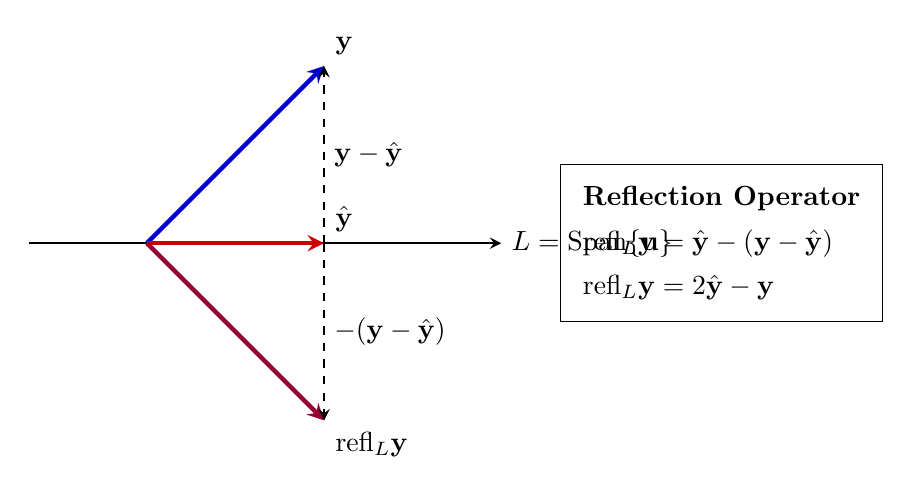
\begin{tikzpicture}[scale=1.5]
    \draw[thick, ->, >=stealth] (-1, 0) -- (3, 0) node[right] {$L = \text{Span}\{\mathbf{u}\}$};
    \coordinate (O) at (0,0);
    \coordinate (Y) at (1.5, 1.5);
    \coordinate (Yhat) at (1.5, 0);
    \coordinate (Refl) at (1.5, -1.5);
    
    \draw[ultra thick, blue!80!black, ->, >=stealth] (O) -- (Y) node[above right, text=black] {$\mathbf{y}$};
    \draw[ultra thick, red!80!black, ->, >=stealth] (O) -- (Yhat) node[above right, text=black] {$\hat{\mathbf{y}}$};
    \draw[ultra thick, purple!80!black, ->, >=stealth] (O) -- (Refl) node[below right, text=black] {$\text{refl}_L \mathbf{y}$};
    
    \draw[thick, dashed, ->, >=stealth] (Yhat) -- (Y) node[midway, right, text=black] {$\mathbf{y} - \hat{\mathbf{y}}$};
    \draw[thick, dashed, ->, >=stealth] (Yhat) -- (Refl) node[midway, right, text=black] {$-(\mathbf{y} - \hat{\mathbf{y}})$};
    
    \node[align=left, anchor=west, draw, inner sep=8pt] at (3.5, 0) {
        \textbf{Reflection Operator}\\[4pt]
        $\text{refl}_L \mathbf{y} = \hat{\mathbf{y}} - (\mathbf{y} - \hat{\mathbf{y}})$\\[4pt]
        $\text{refl}_L \mathbf{y} = 2\hat{\mathbf{y}} - \mathbf{y}$
    };
\end{tikzpicture}
\end{center}

\textbf{44. Matrix $U$ is formed by normalizing columns of $A$. Explain properties of $U^T U$ and $U U^T$.}
\begin{proof}
    (a) $U^T U = I$ because the columns of $U$ are orthonormal. $U U^T$ is the projection matrix onto the column space of $A$, which is not the identity matrix unless $U$ is square. \\
    (b) $\mathbf{p} = U U^T \mathbf{y}$. Since $\mathbf{p} = U (U^T \mathbf{y})$, it is a linear combination of the columns of $U$, so $\mathbf{p} \in \text{Col } A$. \\
    (c) $\mathbf{z} = \mathbf{y} - \mathbf{p}$. $U^T \mathbf{z} = U^T (\mathbf{y} - U U^T \mathbf{y}) = U^T \mathbf{y} - (U^T U) U^T \mathbf{y} = U^T \mathbf{y} - I U^T \mathbf{y} = \mathbf{0}$. Thus, $\mathbf{z}$ is orthogonal to every column of $U$. \\
    (d) Since $\mathbf{z}$ is orthogonal to the columns of $U$ (which span $\text{Col } A$), $\mathbf{z}$ is in the orthogonal complement, $(\text{Col } A)^\perp$.
\end{proof}

\newpage
\section{In-Depth Analysis of Problems and Techniques}

\subsection{Problem Types and General Approach}
\begin{itemize}
    \item \textbf{Orthogonality Verification (Ex 1-6):} The strategy is purely computational. Compute the dot product $\mathbf{u}_i \cdot \mathbf{u}_j$ for all distinct pairs. If any product is non-zero, the set is not orthogonal.
    \item \textbf{Orthogonal Basis Expansion (Ex 7-10):} Instead of setting up an augmented matrix and row-reducing to find weights $c_1, c_2, \dots$, we exploit the orthogonal basis theorem. The weight for vector $\mathbf{u}_i$ is simply $c_i = \frac{\mathbf{x} \cdot \mathbf{u}_i}{\mathbf{u}_i \cdot \mathbf{u}_i}$.
    \item \textbf{Projections and Distances (Ex 11-16):} These problems require decomposing a vector $\mathbf{y}$ into $\hat{\mathbf{y}}$ (the projection) and $\mathbf{z}$ (the orthogonal component). The distance from $\mathbf{y}$ to the subspace is the norm of the error vector, $\|\mathbf{z}\|$.
    \item \textbf{Matrix Properties (Ex 33-44):} These are theoretical proofs relying on the definition of matrix multiplication and transposes. The core trick is recognizing that the $(i,j)$-entry of $U^T U$ is exactly the dot product of the $i$-th and $j$-th columns of $U$.
\end{itemize}

\subsection{Key Algebraic and Calculus Manipulations}
\begin{itemize}
    \item \textbf{The Transpose Trick for Dot Products:} The dot product $\mathbf{u} \cdot \mathbf{v}$ can be written as the matrix multiplication $\mathbf{u}^T \mathbf{v}$. This is crucial for proving matrix properties, such as $\|U\mathbf{x}\|^2 = (U\mathbf{x})^T (U\mathbf{x}) = \mathbf{x}^T U^T U \mathbf{x}$.
    \item \textbf{Scalar Pull-Out in Projections:} When projecting onto $c\mathbf{u}$, the scalar $c$ cancels out: $\frac{\mathbf{y} \cdot (c\mathbf{u})}{(c\mathbf{u}) \cdot (c\mathbf{u})} (c\mathbf{u}) = \frac{c(\mathbf{y} \cdot \mathbf{u})}{c^2(\mathbf{u} \cdot \mathbf{u})} c\mathbf{u} = \frac{\mathbf{y} \cdot \mathbf{u}}{\mathbf{u} \cdot \mathbf{u}} \mathbf{u}$. This proves that projection depends only on the \textit{line} (span), not the specific vector chosen.
\end{itemize}

\section{Cheatsheet and Tips for Success}

\textbf{Core Formulas:}
\begin{itemize}
    \item \textbf{Orthogonal Projection:} $\text{proj}_{\mathbf{u}} \mathbf{y} = \frac{\mathbf{y} \cdot \mathbf{u}}{\mathbf{u} \cdot \mathbf{u}} \mathbf{u}$
    \item \textbf{Orthogonal Decomposition:} $\mathbf{y} = \hat{\mathbf{y}} + \mathbf{z}$, where $\mathbf{z} = \mathbf{y} - \hat{\mathbf{y}}$
    \item \textbf{Orthogonal Matrix Condition:} $U^T U = I$
\end{itemize}

\textbf{Tips and Tricks:}
\begin{itemize}
    \item \textbf{The Zero Vector Trap:} The zero vector is orthogonal to \textit{everything}. A set containing the zero vector can be an orthogonal set, but it will \textit{never} be linearly independent, and it can \textit{never} be an orthonormal set (since its norm is 0, not 1).
    \item \textbf{Check Your Projections:} You can always verify if your projection $\hat{\mathbf{y}}$ is correct by computing the dot product of $\mathbf{z} = \mathbf{y} - \hat{\mathbf{y}}$ with $\mathbf{u}$. If $\mathbf{z} \cdot \mathbf{u} \neq 0$, you made an arithmetic error.
    \item \textbf{Square vs. Non-Square Matrices:} If $U$ is $m \times n$ with orthonormal columns, $U^T U = I_n$. However, $U U^T$ is \textit{only} the identity matrix if $U$ is square ($m=n$). Otherwise, $U U^T$ is a projection matrix.
\end{itemize}

\newpage
\section{Conceptual Synthesis and The "Big Picture"}

\subsection{Thematic Connections}
The core theme of this topic is \textbf{decoupling}. In standard coordinate systems, changing one variable might affect the others. By using an orthogonal basis, the axes are completely independent. This is the exact same principle used in \textbf{Fourier Series} in calculus, where functions are projected onto an infinite-dimensional orthogonal basis of sine and cosine waves. Because the sine and cosine functions are orthogonal under the integral inner product $\int_{-\pi}^{\pi} f(x)g(x) dx$, we can compute Fourier coefficients independently, exactly like the weights $c_j$ in Theorem 5.

\subsection{Forward and Backward Links}
\begin{itemize}
    \item \textbf{Backward:} This topic builds directly on the dot product and the Pythagorean theorem. The distance formula $\|\mathbf{y} - \hat{\mathbf{y}}\|$ is simply the Pythagorean theorem applied to $n$-dimensional space.
    \item \textbf{Forward:} Understanding orthogonal projections is the absolute bedrock for \textbf{Least Squares Regression} (Section 6.5). When a system $A\mathbf{x} = \mathbf{b}$ has no solution, we project $\mathbf{b}$ onto the column space of $A$ to find the "closest possible" solution. It is also the foundation for the \textbf{Gram-Schmidt Process} and \textbf{Principal Component Analysis (PCA)}.
\end{itemize}

\section{Abstract Real-World Modeling (AI, ML, \& Quant Finance)}

\subsection{Concrete Scenarios}
1. \textbf{Quantitative Finance (Factor Models):} In Arbitrage Pricing Theory (APT), asset returns are modeled as linear combinations of orthogonal risk factors. If the factors are orthogonalized (using PCA), the covariance matrix becomes diagonal, drastically simplifying portfolio optimization and risk management.
2. \textbf{Machine Learning (Ordinary Least Squares):} In predictive modeling, we often have more data points than features (an overdetermined system). The OLS estimator finds the hyperplane that minimizes the sum of squared residuals, which is geometrically equivalent to projecting the target vector $\mathbf{y}$ orthogonally onto the column space of the feature matrix $X$.

\subsection{Model Problem Setup: OLS in Statistical Learning}
Let $X \in \R^{N \times p}$ be a design matrix of $N$ observations and $p$ features, and $\mathbf{y} \in \R^N$ be the target vector. We assume $\mathbf{y} \notin \text{Col}(X)$. We seek a weight vector $\boldsymbol{\beta} \in \R^p$ that minimizes the loss function:
\[ \mathcal{L}(\boldsymbol{\beta}) = \|\mathbf{y} - X\boldsymbol{\beta}\|^2 \]
Geometrically, $X\boldsymbol{\beta}$ is a vector in $\text{Col}(X)$. The minimum distance occurs when the residual vector $\boldsymbol{\epsilon} = \mathbf{y} - X\boldsymbol{\beta}$ is orthogonal to every column of $X$. 
This orthogonality condition requires that $X^T \boldsymbol{\epsilon} = \mathbf{0}$.
\begin{align*}
    X^T (\mathbf{y} - X\boldsymbol{\beta}) &= \mathbf{0} \\
    X^T \mathbf{y} - X^T X \boldsymbol{\beta} &= \mathbf{0} \\
    X^T X \boldsymbol{\beta} &= X^T \mathbf{y}
\end{align*}
These are the famous \textbf{Normal Equations}. If the columns of $X$ were an orthonormal basis, then $X^T X = I$, and the optimal weights would simply be $\boldsymbol{\beta} = X^T \mathbf{y}$, perfectly mirroring Theorem 5!

\newpage
\section{Common Variations and Untested Concepts}

\subsection{The Gram-Schmidt Process}
The homework tests if a set is orthogonal, but it does not ask you to \textit{create} an orthogonal set from a non-orthogonal one. The Gram-Schmidt process does exactly this.
\textbf{Example:} Given $\mathbf{x}_1 = \begin{bmatrix} 1 \\ 1 \end{bmatrix}$ and $\mathbf{x}_2 = \begin{bmatrix} 0 \\ 2 \end{bmatrix}$, find an orthogonal basis.
\begin{align*}
    \mathbf{v}_1 &= \mathbf{x}_1 = \begin{bmatrix} 1 \\ 1 \end{bmatrix} \\
    \mathbf{v}_2 &= \mathbf{x}_2 - \text{proj}_{\mathbf{v}_1} \mathbf{x}_2 = \begin{bmatrix} 0 \\ 2 \end{bmatrix} - \frac{2}{2} \begin{bmatrix} 1 \\ 1 \end{bmatrix} = \begin{bmatrix} -1 \\ 1 \end{bmatrix}
\end{align*}
The set $\{\mathbf{v}_1, \mathbf{v}_2\}$ is now an orthogonal basis.

\subsection{Projection Matrices}
The homework touches on $U U^T$, but formally, the matrix $P = A(A^T A)^{-1} A^T$ is the standard projection matrix onto the column space of $A$. If $A$ has orthonormal columns (let's call it $U$), then $U^T U = I$, and the formula collapses beautifully to $P = U U^T$.

\section{Advanced Diagnostic Testing: "Find the Flaw"}

Below are 5 flawed solutions. Act as the grader: find the error, explain it, and provide the correct solution.

\textbf{Problem 1:} Find the projection of $\mathbf{y} = \begin{bmatrix} 3 \\ 4 \end{bmatrix}$ onto $\mathbf{u} = \begin{bmatrix} 1 \\ 2 \end{bmatrix}$.
\textit{Flawed Solution:} $\hat{\mathbf{y}} = \frac{\mathbf{y} \cdot \mathbf{u}}{\mathbf{y} \cdot \mathbf{y}} \mathbf{u} = \frac{3+8}{9+16} \begin{bmatrix} 1 \\ 2 \end{bmatrix} = \frac{11}{25} \begin{bmatrix} 1 \\ 2 \end{bmatrix}$.
\begin{itemize}
    \item \textbf{Error:} The denominator uses $\mathbf{y} \cdot \mathbf{y}$ instead of $\mathbf{u} \cdot \mathbf{u}$.
    \item \textbf{Correction:} $\hat{\mathbf{y}} = \frac{\mathbf{y} \cdot \mathbf{u}}{\mathbf{u} \cdot \mathbf{u}} \mathbf{u} = \frac{11}{5} \begin{bmatrix} 1 \\ 2 \end{bmatrix} = \begin{bmatrix} 11/5 \\ 22/5 \end{bmatrix}$.
\end{itemize}

\textbf{Problem 2:} Check if $\mathbf{v}_1 = \begin{bmatrix} 1 \\ -1 \end{bmatrix}$ and $\mathbf{v}_2 = \begin{bmatrix} 1 \\ 1 \end{bmatrix}$ form an orthonormal set.
\textit{Flawed Solution:} $\mathbf{v}_1 \cdot \mathbf{v}_2 = 1 - 1 = 0$. Since they are orthogonal, they are orthonormal.
\begin{itemize}
    \item \textbf{Error:} The solution fails to check if the vectors have unit length.
    \item \textbf{Correction:} $\|\mathbf{v}_1\| = \sqrt{2} \neq 1$. The set is orthogonal, but \textit{not} orthonormal.
\end{itemize}

\textbf{Problem 3:} Let $U = \begin{bmatrix} 1 & 1 \\ 0 & 1 \end{bmatrix}$. Compute $U^T U$.
\textit{Flawed Solution:} Since $U$ is a square matrix, $U^T U = I$.
\begin{itemize}
    \item \textbf{Error:} The theorem $U^T U = I$ only applies if $U$ has \textit{orthonormal columns}. The columns of this $U$ are not orthogonal ($1 \cdot 1 + 0 \cdot 1 = 1 \neq 0$).
    \item \textbf{Correction:} $U^T U = \begin{bmatrix} 1 & 0 \\ 1 & 1 \end{bmatrix} \begin{bmatrix} 1 & 1 \\ 0 & 1 \end{bmatrix} = \begin{bmatrix} 1 & 1 \\ 1 & 2 \end{bmatrix}$.
\end{itemize}

\textbf{Problem 4:} Find the distance from $\mathbf{y} = \begin{bmatrix} 2 \\ 2 \end{bmatrix}$ to the line spanned by $\mathbf{u} = \begin{bmatrix} 1 \\ 0 \end{bmatrix}$.
\textit{Flawed Solution:} $\hat{\mathbf{y}} = \frac{2}{1} \begin{bmatrix} 1 \\ 0 \end{bmatrix} = \begin{bmatrix} 2 \\ 0 \end{bmatrix}$. The distance is $\|\hat{\mathbf{y}}\| = 2$.
\begin{itemize}
    \item \textbf{Error:} The distance to the subspace is $\|\mathbf{y} - \hat{\mathbf{y}}\|$, not $\|\hat{\mathbf{y}}\|$.
    \item \textbf{Correction:} $\mathbf{z} = \mathbf{y} - \hat{\mathbf{y}} = \begin{bmatrix} 2 \\ 2 \end{bmatrix} - \begin{bmatrix} 2 \\ 0 \end{bmatrix} = \begin{bmatrix} 0 \\ 2 \end{bmatrix}$. Distance $= \|\mathbf{z}\| = 2$. (The numerical answer was coincidentally the same, but the logic was fatally flawed).
\end{itemize}

\textbf{Problem 5:} Express $\mathbf{x} = \begin{bmatrix} 1 \\ 5 \end{bmatrix}$ as a linear combination of $\mathbf{u}_1 = \begin{bmatrix} 1 \\ 1 \end{bmatrix}$ and $\mathbf{u}_2 = \begin{bmatrix} 1 \\ 2 \end{bmatrix}$.
\textit{Flawed Solution:} $c_1 = \frac{\mathbf{x} \cdot \mathbf{u}_1}{\mathbf{u}_1 \cdot \mathbf{u}_1} = \frac{6}{2} = 3$. $c_2 = \frac{\mathbf{x} \cdot \mathbf{u}_2}{\mathbf{u}_2 \cdot \mathbf{u}_2} = \frac{11}{5}$. So $\mathbf{x} = 3\mathbf{u}_1 + \frac{11}{5}\mathbf{u}_2$.
\begin{itemize}
    \item \textbf{Error:} The projection formula for weights only works if the basis is \textit{orthogonal}. $\mathbf{u}_1 \cdot \mathbf{u}_2 = 3 \neq 0$.
    \item \textbf{Correction:} You must solve the system $\begin{bmatrix} 1 & 1 \\ 1 & 2 \end{bmatrix} \begin{bmatrix} c_1 \\ c_2 \end{bmatrix} = \begin{bmatrix} 1 \\ 5 \end{bmatrix}$. Row reduction yields $c_1 = -3, c_2 = 4$.
\end{itemize}

\end{document}